\chapter{后记}
\section{初稿}
2018年10月23日

写这本笔记大概花了我两个月的时间,此时这本笔记大概有200千字(50千字为中文),我
为自己的成果感到骄傲。在此期间我系统地复习了NOIP复赛以上的知识点,学到了许多新的方法/技巧/
思路,重新理解了之前看不懂的算法,收获颇多。我将自己的想法记录于此,以便之后重新翻阅。
该笔记在内容上还是较为完整的,在接下来的时间内我会在巩固的过程中继续学习并补充新的高级算法
/数据结构,以应战省选和NOI2019。

在我作为D类队员参加了NOI2018现场赛后,我发现了自己的严重问题------知识点掌握不扎实,
导致我没能拿到该得的分数。所以我决定自己写一写复习笔记来建立出一套自己的思维体系。

同时作为目前校内在OI道路上走的最远的人(其他人初赛都过不了。。。孤单),我没有
信息学强校学生所拥有的资源——学长。有学长的指导和遗留下的资料,能够少走许多弯路。
既然自己没有学长,只好自己做学长了。这本笔记算是是我的一份心意吧,希望学校的OI事业
能够有所发展,学弟们(???我好像根本不知道有学弟)如果需要我帮助的地方,随时联系我。
我的表达能力不太好,而且有些简单的地方没有细讲,你们可以打开页底下的参考资料链接细看
(这些资料是我自己能够接受并理解的),虽然这些东西在百度和维基上都能轻易找到,但我之前
根本就不知道这些东西的存在(直到考完后才知道,已经晚了)。。。所以你们就把它当做一种索引吧。

在写这本笔记的过程中,我发现自己在使用\LaTeX{}和排版方面还存在许多问题:
\begin{itemize}
    \item 目录太长,分类过细
    \item 参考资料链接过多
    \item 不恰当的知识点分类
    \item 过长的TODO List
    \item 滥用lstlisting
    \item 书籍排版密度过低
    \item 滥用Index
    \item 未熟练使用BibTex
    \item 数学公式排版掌握不熟
    \item 缺少图片
    \item 语言表达不当或过于口语化(才发现``即可''之类的词是从其它blog上学来的)
\end{itemize}

上述问题将会在接下来几轮的review中得到改善。

在此我要感谢学校领导、老师和同学的理解与支持,感谢父母(还有我妹)对我的
大力支持。感谢写出优秀博客的OIers和Wikipedia-EN的维护者,他们为我提供了大量的
参考资料与经验总结,使我受益匪浅,我所做的不过是将它们聚集在一块而已。
\CJKsout{差点忘了感谢CCF}。

刚开始写这本笔记时,我遇到了一件让我感到最幸福的事:我喜欢的女生向我表白了。
在此之前我已经预先认真考虑了几个月,所以当时我毫不犹豫就接受了。那个月是我最幸福的日子,
我开始改变自己,更加努力地学习,以应对将来需要承担的责任。她给了我写这本笔记的动力,她能够
理解许多别人所不能理解我的事情。我当时认为自己是这个世上最幸运的人。但好景不长,在本笔记
初稿即将完成时,我最担心的事情还是发生了——双方突然无话可说。我是预先知道这个问题会发生,
而且已经预先提醒过她了——遇到问题要多沟通,商量解决方案。但在短短几天内,她对我的态度越来
越差。最后她以一堆自相矛盾的理由离开了我,根本不给我与之沟通的机会。从前的誓言,以及我对
她的好,她似乎已经完全忘记了。我不知道她的真实意图,她或许是为了让我安心学习。我仍然相
信自己的单元测试是可靠的,她最终会回来的。我决定履行自己之前的诺言:我等她两年。我好想在
她身边给她讲解数学题;好想在她生理期时给她端杯热水,陪在她身边;好想和她一起去公园散步,
在绿道慢跑,一起看动画电影;好想在她心情不好时,自己在旁边给她疏导,给她一个拥抱;好想
静静地坐在一旁,听她弹琴唱歌;好想再让她笑着敲我的头;好想高中毕业后用自己的Renderer给她
渲一个鸽了两年的生日礼物。唉,这些愿望怕是无法实现了。现在自己还是先努力学习,认真搞OI,
考上理想的大学。\CJKsout{得之我幸,不得我命。未来会怎么样,得看自己的造化了。}
{\bfseries I can do it!}

$\frac{\sin 4\theta}{\sin \theta}$,我等你回来。

\section{二轮复习}
2019年1月3日

不得不吐槽Review花的时间居然比编写还要久。。。

二轮复习后我对该笔记做了大量修改,主要内容如下:

\begin{itemize}
    \item 补充了大量高级内容
    \item 补充了刷题过程中的一些解题方法、坑点
    \item 修改了一些不恰当、不详细的文字表述
    \item 更正文中错误
    \item 规范符号与术语的表达
    \item 解决并同时新增了一些TODO
    \item \CJKsout{消灭了``即可''}
\end{itemize}

NOIP2018已经过去了,我初赛成绩86,复赛成绩496,成绩还算令人满意(这里的人指老师、
校领导和局领导们)。虽然我能凭这个成绩去WC2019和THUWC2019,但是我知道自己的实力仍然不够。
NOIP2018暴露了我的另外一个问题:粗心。初赛因两题水题而不能AK,复赛因没有从理论上论证算法
正确性而留下成绩不能上500的遗憾(感谢CCF负责任的数据)。根本原因仍然是我对知识点的掌握不够
熟练。

我接下来的规划:

\begin{itemize}
    \item 针对薄弱专题继续复习与刷题。
    \item 巩固新学的知识。
    \item 在WC2019后继续学习新知识。
    \item 参加线上比赛以提高应试能力和分析思考能力
    \item 学会使用Vim,提高码速
\end{itemize}

在此我也总结一下我的2018吧。
\begin{itemize}
    \item 2018年,我结识了一些OIer,见识了各类型比赛,意识到自己的水平很菜。
    \item 2018年,我借助CUDA写了一个玩具级光栅化渲染器/基于物理的渲染器,感受到了
    CG的魅力,以及其幕后需要的大量数学/物理知识储备。
    \item 2018年,我经历了从年段第2一路跌到年段第九十几名,再一路从60,30,15回到
    年段第2的``过山车''式的惊险。在此感谢我的老师对我的鼓励,段长对我的教导,以及她
    在那段时间对我的支持与鼓励。
    \item 2018年,我经历了从喜欢到恋爱,再到失恋的标准早恋结局(事实上我的遭遇比
    早恋要惨得多)。我仍然等着她,因为我对她有承诺,对自己也有承诺。
    \item 2018年,我发现自己的计算机/OI/数学知识可以应用到许多方面,包括但不限于:
    \begin{itemize}
        \item 物理探究课上给使用传感器的物理实验设备安装驱动\CJKsout{,然后被物理老师
        当做苦力给每台机子都安装一遍}
        \item 给班里的英语剧做音频剪辑
        \item 被地理老师请去给机器人编程
        \item 用扒注册表的手段清除了班班通的病毒(顺便安利了一波火绒杀毒)
        \item 给数学老师和同学们安利了一波GeoGebra(垃圾几何画板)
        \item 在语文课上放映用\LaTeX{}做的\CJKsout{ppt}beamer,惊艳全场
        \item 在英语课上高举《线性代数及其应用》给老师讲``列''的单词应该是column
    \end{itemize}
    \item 到了年底,感觉到自己的身体快撑不住了(或许是因失恋而过度伤心)。
    于是我提早了运动计划的实施(本来想在退役后才开始的),坚持每天晨跑。一个星期后,
    困扰我多年的过敏性鼻炎有了好转。至此以后我上课更加精神了,因此被英语老师表扬。
    上个星期我还被路上的一位老人表扬了,继续坚持!!!
\end{itemize}

没有她的这段时间里,起初我是十分痛苦的。我的人生计划第二次被她打断,原来幻想的幸福美满
的家庭成了泡影。那段时间我一直都在听Right Here Waiting。后来我意识到再这样颓废下去,
不仅这个梦想破灭了,另一个梦想也将受到影响。如果这两个梦想能够实现一个,我就很满足了。
偶然有一次我听到《中国男儿》后,更加坚定了改变自己的决心。我第一次听这首歌是在电视剧
《五星红旗迎风飘扬》中。片尾氢弹爆炸的场景,以及这首歌的旋律和歌词,给我的印象很深。

歌词一起放在这里:
\begin{center}
中国男儿,中国男儿,要将只手撑天空。\\
睡狮千年,睡狮千年,一夫振臂万夫雄。\\
长江大河,亚洲之东,峨峨昆仑,翼翼长城,\\
天府之国,取多用宏,黄帝之胄神明种。\\
风虎云龙,万国来同,天之骄子吾纵横。\\
中国男儿,中国男儿,要将只手撑天空。\\
睡狮千年,睡狮千年,一夫振臂万夫雄。\\
我有宝刀,慷慨从戎,击楫中流,泱泱大风,\\
决胜疆场,气贯长虹,古今多少奇丈夫。\\
碎首黄尘,燕然勒功,至今热血犹殷红。\\
中国男儿,中国男儿,要将只手撑天空。\\
睡狮千年,睡狮千年,一夫振臂万夫雄。\\
长江大河,亚洲之东,峨峨昆仑,翼翼长城,\\
天府之国,取多用宏,黄帝之胄神明种。\\
风虎云龙,万国来同,天之骄子吾纵横。\\
\end{center}

前几天我又看了《中国面壁者》,感触很深。或许这才是我的归宿吧。

她提出分手前,我正在对她的感情稳定性进行测试(我是个奇怪的\CJKsout{人}计算机)。
当她说出我们已经无话可聊时,我的内心是欣慰的。我努力了这么久,终于构造出了一个
极端条件,这是一个很好的锻炼机会。但是她的下一句``分吗''如同晴天霹雳。既然她不喜欢我
也不再理我了,我的测试也变得既没有意义也不能实行。我只能努力改变自己,做好充分准备,
抓住一切机会。

出了这档子事,我的职业选择也不再局限于NVIDIA那种自由的工作了,本来想多陪陪家人的。
现在我感兴趣的职业方向如下:
\begin{itemize}
    \item CG:Disney的动画电影对我影响很深,所希望自己的技术能够协助
    电影艺术家创作出优秀的动画电影,向世人宣传正能量
    \item HPC:指挥一堆CPU协作和指挥千军万马一样浪漫
\end{itemize}

一言难尽啊。。。。适可而止吧,睡觉时间快到了。

比赛在即,我要更加努力。

THUWC2019\&WC2019\&FJOI2019 Round 1加油!!!

\section{三轮复习}
2019年4月4日

一轮更比一轮咕。

这三个月来我对该笔记做了大量修改,主要内容如下:

\begin{itemize}
    \item 补充了一些学习计划外的技巧(\CJKsout{需求刺激进步})
    \item \CJKsout{升级了Checker}
    \item \CJKsout{将某些连自己都看不懂的文字表述修改为
    将来的我看不懂的文字表述}
    \item 准备对解题思路程序化,添加了几类问题的系统解题思路。
    未来可能会做思维导图?
\end{itemize}

再记一下上一轮复习牵挂的事:

\begin{itemize}
    \item THUWC2019:进了面试,口语测试体验极差(\CJKsout{老师你刚才只叫我读啊,
    我就一个单词一个单词地念啊。老师:好了你可以出去了。}),拿到了神奇的三等约:
    再来一次。
    \item WC2019:冬眠营果然名不虚传,我从去广州开始一直睡到了FJWC2019。考试体验
    极差,交互题暴零又让我拿了一次Cu(要是CTSC2018没有Day3我就可以达成集齐NOI系列
    赛事Cu的成就了,可惜今年为了不浪费时间没报CTSC和APIO)。考试前还被去年CTSC/APIO
    的室友嘲笑了一番:你怎么看起来这么落寞啊。在考试前知道了他去年PKUWC已经签了无条件
    本一,进考场时心里很不是滋味。
    \item FJOI2019 Round 1:鸽到和FJOJ2019 Round 2一起进行,还有一个星期左右。
    不过从FJWC2019的模拟成绩来看,我连D类都够不着。
    \item 她:与我不再有任何联系,不过看她的学习和生活没有受到任何影响我也就放心了。
\end{itemize}

接下来的计划:
\begin{itemize}
    \item 完成系统解题思路梳理,把会的东西全部挂上去,不熟的东西舍弃掉。
    \item 继续按照专题刷题。
    \item 从头开始Review(下一次后记的时间会不会咕到退役?)。
    \item 省选后开始看集训队论文。
    \item 刷各大赛事的题目。
\end{itemize}

她离开后我感觉心里空落落的,有开心的事没有人分享,受到了打击也没有人安慰。再加上这一个
月多都在家里,每天除了吃饭睡觉散步,其它时间都待在电脑面前,一天没说几句话。我感觉自己
快要疯了,白天有时会摸鱼看新闻写Checker,晚上有时候写题写到一点多(有时在写Checker),
在自己房间里会颓废看视频,会一个人和自己用记事本聊天,会一个人缩在被子里泣\CJKsout{
(《水浒传》~第二十五回~王婆计啜西门庆~淫妇药鸩武大郎:看官听说:原来但凡世上妇人,哭有
三样:有泪有声谓之哭,有泪无声谓之泣,无泪有声谓之号。)}。我不知道再这样下去自己的生理
和心理会不会崩溃,写初稿的第一个月自己可不是这样的。只能强制自己死撑了,崩溃了也算是一种
解脱,只是感觉对不起身边对自己寄予厚望的人们。好怀念那一个月的时光啊,那可能是我最幸福
也是最痛苦的回忆了。

对于她的行为,我不能理解,无法接受,但是必须尊重。一年后的生日礼物按照计划准备,但自己
不想再打扰她,还是自己保存着吧。对于自己的感情,认识她之前我就已经跟自己讲得很清楚,只能
按照自己的承诺继续等。虽然复合的希望渺茫(我也不知道即使她愿意复合,我会不会再次信任她),
但这种来自直觉的决策应该是正确的,我等她两年。

感觉自己离开课堂好久了,有点厌学,根本不知道老师到底在讲什么,我已经没有退路了。
moe又在今年开始缩减自主招生规模,提高要求,更是把我逼到绝境。要是像室友那样早一年
进入面试,或许自己就不会遭受这么多打击了。看着他签了无条件本一后一脸轻松的样子,自己
很是羡慕,这两年省排名在自己左右的人基本都签了,就我只有一张废纸。

目前还有两次机会,我希望自己也能有一个True Ending。
\section{FCS NOI2019随笔}
\subsection{day0}
看着自己的笔记发现自己学了好多,这几天也不知道自己要做什么了。希望有备而来的今年能比
懵逼的去年考得更好。

真的好害怕自己在考场上又想起她。。。只要题目不会做我就会想她,然后崩盘(从NOI2018到
WC2019都有过)。而且现在已经分开了,我再也没办法找她要安慰了。今天晚上再小小地哭一会吧,
明早考试应该情绪会好些。

我感觉自己好奇怪,过着和正常学生不一样的生活。每天在不同计算机的面前切换,一整天很少说话,
在学校也很少参加集体活动,常年失踪,在同学眼里我就是个呆子。

但我想说,OIer/程序猿不是这样的!!!他们也可以多才多艺,也可以有丰富的生活,而不是大家公认的
``人傻钱多死的快''。只不过,我也不是正常的程序猿,我让身边人对程序猿的认知出现了偏差。我到现在
还记得初中毕业班的英语老师说的``不要像那些程序猿一样''

可能这里还有一些心理问题吧。不知道为什么,自托儿所开始就不合群,但是我一直都希望自己能够融入
集体。但我努力学习了,成为了老师眼里的乖孩子,但是换来的只不过是同学们的尊敬(仍然记得一年级
被段霸放过的场景),而不是关注。为了刷点存在感,我经常用超出课程的数学来给同学们讲题,但是我
看到的不是同学对未知的渴望,而是在讲台下各做各的。有时甚至连老师都没听,一个好的idea就这样被
埋没了,变成了我的个人表演。现在我在想出一个idea后,也不大愿意与大家分享了,自己晚上回去哭一
哭吧,祭奠一下它。分手前想给她做的题,在分手后18天我终于想出了一个绝妙的纯几何方法,可惜连这个
唯一的听众也离我而去。

所以我的心理才很脆弱啊。如果外校OIer对我防备,对我不理不睬,或者是父母说我这不会那不会,我会哭
一晚上。但如果有人对我很好,关心我(比如她),我可以给出一生的承诺。那是我第一次收到生日礼物,
那是我第一次与女生有长时间的对话,那是我第一次能够把自己的糗事分享出来,那是我第一次去关心一个人
的爱好。这就是喜欢的感觉?但是现在不存在了,那些是第一次,也可能是最后一次。

我实在是不理解,为什么她会把生活过的精彩说得这么容易。在高一,唯一可以调剂我的生活的,只有与
她聊天和捣鼓CG,在高一末被段长劝退CG后,她就是我的唯一。我也考虑过,在自己没有自己的爱好后,就会
对她特别依赖,这会导致不正常的结果。在她表白前也以影响学习为由询问她要不要暂停接触。可最后还是没有
狠下心,造成了现在这个尴尬的局面。我不后悔自己喜欢她,但很疑惑当初为什么她会喜欢我。

有的时候我在想,自己为什么会呆在计算机面前,而不是像正常高中生一样过着精彩的生活。最让人伤心的,
莫过于别人在科技文体艺术节、在元旦晚会上唱歌,而我却在机房里刷题。就算我去参与这些活动也做不好,
现在的我,离开了计算机,什么都不是。\CJKsout{给我一台计算机,我什么都能干!}

可能身边人都觉得我状态很好(没人发现我失恋了),天天乐呵呵的,但他们不知道我在被子里因为一些人
的不理睬、防备、嫌弃哭了多久才假装自己很正常。

好羡慕debug18,能和女朋友一起上THU\url{http://debug18.com/posts/my-2018/}。

好羡慕zhblue,能够引导自己的孩子探寻未知\url{http://www.hustoj.com/?p=1331}。

但对于我,她离开后,这些梦可能都无法实现了。但我希望自己的QQ头像永远不换。

希望这些东西在deadline之前不要被她知道,不希望因为这个而影响她对自己幸福的选择,不过或许这些
东西只会让大家觉得我更幼稚罢了。

\CJKsout{似乎跑题了。。。这是我的书,只要不是政治敏感的东西,爱写啥写啥。好像只有第一行与标题有关。}
\subsection{day1}
凉凉。。。没有一题会写,沦为暴力选手。退役预定。

上天真的要捉弄我吗?我昨晚还说考试时不要想起她,今天外面就响起了她唱过的歌。。。特大声。
外面下着大雨,与我的处境差不多吧。

机会越来越少了,希望越来越渺茫。继续踏实干吧。
\subsection{day1下午}
居然只有5分。。。NOIP那一点优势完全不存在了。省选就像玩一样。退役已定,可以准备好迎接
惨淡的人生了。

她。。。复合的概率只剩下bias了吧。

晚上不知又要哭多久。。。

人生没有Debug啊,不能断点,不能单步,像是并发。

我不知道自己还能撑多久,在被宣判死刑前,把自己一直以来的梦说出来吧。

\begin{itemize}
    \item 有一个稳定和谐的家庭
    \item 捣鼓CG
    \item 有空时在县里开班招生,造学弟
    \item 吃吃吃
\end{itemize}

全凉了。

晚上学点Rust放松一下,明天可能没心情考试了吧。
\subsection{day2}
为什么前两题这么水。。。对于这套题目我一点优势都没有。

果然一堆人200+。

退役。老爸的Plan B也该泡汤了罢。

两个月的养老生活结束了,再也不能待在家人身边。自己的猜想果然不错,校领导知道没戏后,
就叫我滚回去学文化课了。

混了两年换来这个结果。不仅没得到想要的,还失去了许多。。。这就是人生?
\section{End}
2019年5月20日

最后一次比赛后我就再也碰不了电子设备了,所以这里提前做个收尾。

THUSC2019应该是我OI生涯中的最后一站吧。我也大概知道了结局,否则也不会花一个月的时间搞
THUAC,甚至抽时间刷电影,这两个是我一直想做但忍着不做的事。

我没能达到自己的要求,既不能留住她,也不能让自己走出失恋的阴影,从而丧失刷题的动力。

我还有一堆的TODO没有做完,如果我能撑到高中毕业而没有崩溃的话,我会抽时间完成它的。但是不
再加入新的东西。如果有学弟愿意接手这个烂摊子,可以发Pull Request给我。

至于开班造学弟的事情,由于我可能上不了很好的大学,会成为反面教材,并且加上近年来moe对
竞赛方面自主招生的打压,应该不会有家长送人来,学校也不会配合的。我能留给学弟的,只有这
本笔记,附赠一个Checker。

送给学弟们的忠告:
\begin{itemize}
    \item 适当地娱乐,要注意调整比例。我当时靠着鼓捣CG还能保持0娱乐,离开它后整个人
    就变得毫无生气,离开她后就开始颓废。
    \item 尽量组团学习,同等级OIer之间的交流可以大量节约时间,而且不会感到孤独。
    \item 我在笔记中标记的坑,一定要记住。这是我用时间与分数换来的。
    \item 多训练思维。在掌握笔记中的知识后,你们能做的只有裸题而已。要思考如何将考点隐藏,
    如何转化。
    \item 多出题。上面一条我也做不到,因为我能接触到的题目少。如果你们是组团学习的,可以考虑
    互相出题,互相Hack,这同样是一种训练。多Hack可以熟悉出题人可以怎样卡掉某个算法。
    \item 多打比赛。平时训练和比赛时的心理与策略是十分不同的。缺少比赛也是我的不足。
    \item 所以说,只要人数多,你们就可以自己出题,举办校赛,赛后hack,这样的训练效果比我自己
    一个人刷题好得多。
    \item 同样重视数学和编程方面的训练。虽然OI侧重于算法设计,但是数学功底好就可以快速
    推导式子,提高对语言的掌握程度可以减少bug。
    \item 如果有事找我,请确保你的C++代码大括号不换行。其它的代码风格我可以兼容,但是大括号
    免谈。
\end{itemize}

希望将来我校有人能完成我未能完成的梦想,最好能挑大梁,培养更多的学弟学妹。

希望这本笔记对你们有一些帮助。

\begin{figure}
    \centering
    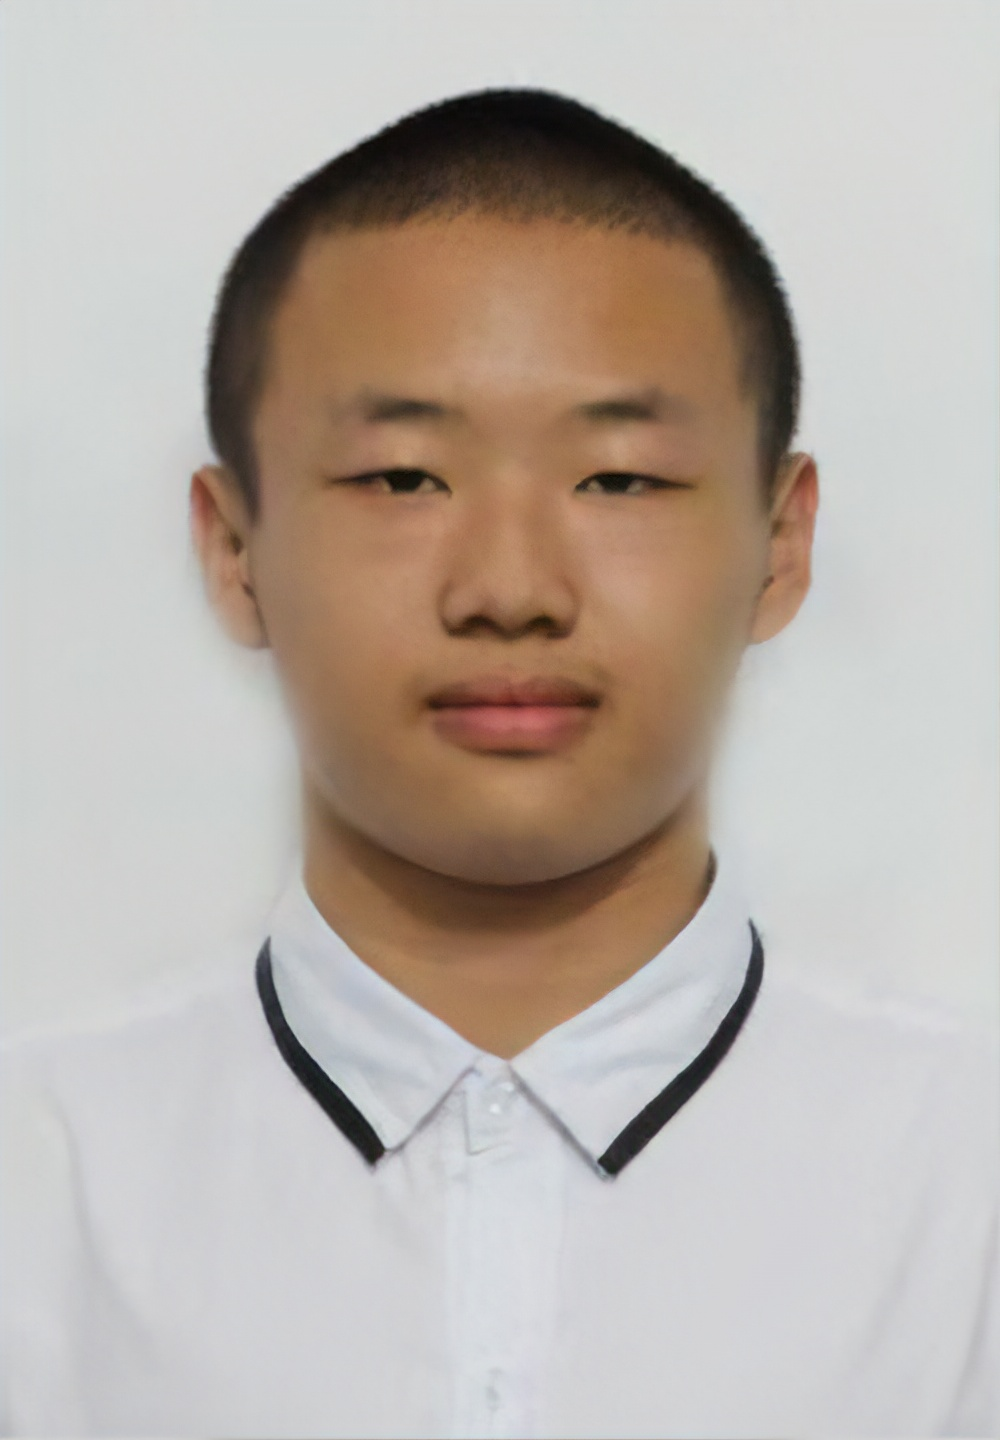
\includegraphics[width=0.8\textwidth,clip]{mypic.jpg}
    \caption{这应该是本笔记唯一一张图了}
\end{figure}
